\documentclass{beamer}
%
% Choose how your presentation looks.
%
% For more themes, color themes and font themes, see:
% http://deic.uab.es/~iblanes/beamer_gallery/index_by_theme.html
%
\mode<presentation>
{
  \usetheme{default}      % or try Darmstadt, Madrid, Warsaw, ...
  \usecolortheme{default} % or try albatross, beaver, crane, ...
  \usefonttheme{default}  % or try serif, structurebold, ...
  \setbeamertemplate{navigation symbols}{}
  \setbeamertemplate{caption}[numbered]
} 

\usepackage[english]{babel}
 % \usepackage[utf8x]{inputenc}
\usepackage[style=authoryear]{biblatex}
\addbibresource{references.bib}
\usepackage{tikz}
\graphicspath{{figures/}}
\DeclareMathOperator{\sign}{sign}

\usepackage{caption}
\captionsetup{font=scriptsize, labelfont=scriptsize}

\title[Your Short Title]{When does atmospheric dryness drive or reduce evapotranspiration?}
\author{Adam Massmann,  Pierre Gentine and Changjie Lin}
\institute{EEE Graduate Student Symposium}
\date{October 27th, 2017}

\begin{document}

\begin{frame}
  \titlepage
\end{frame}


\section{Introduction}
\begin{frame}{When does atmospheric dryness (VPD) drive or reduce evapotranspiration (ET)?}
  \begin{Huge}
  \[VPD = (1-RH)\cdot e_s (T)\]
\end{Huge}
  \begin{itemize}
  \item \textbf{Hydrometeorologists} would say that an increase in VPD (increase in \textbf{atmospheric demand}) would drive an \textbf{increase in ET}.
  \end{itemize}
\end{frame}

\begin{frame}%{When does atmospheric dryness (VPD) drive or reduce evapotranspiration (ET)?}
  \begin{figure}
  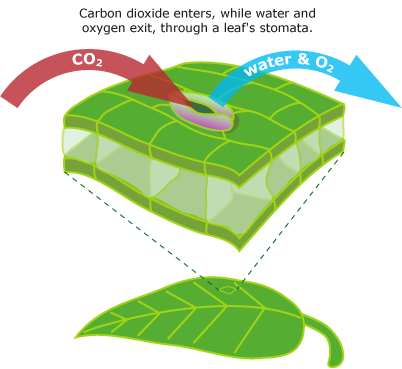
\includegraphics[width=2.70in]{stomata.png}% was O(1.5in)
  \caption{from evolution.berkeley.edu}
\end{figure}
  \begin{itemize}
  \item However, \textbf{plant physiologists} know that plants have evolved to use stomata to conserve and regulate water use. So \textbf{stomata closure} in response to increases in VPD may \textbf{decrease ET}.
  \end{itemize}
\end{frame}


\begin{frame}{The question is, which effect dominates with an increase in VPD: plant response (decrease in ET) or atmospheric demand (increase in ET)?}
  \begin{itemize}
  \item It should be a function of plant type and the environment:
    \begin{itemize}
    \item Plants that are evolved to conserve water will tend to reduce ET with increases in VPD.
    \item However the environment can overwhelm plant response: at some threshold (i.e. very high VPD) the atmospheric demand should dominate and plants will not be able to conserve water, no matter how much they have evolved to do so.
    \end{itemize}
  \end{itemize}
\end{frame}
% develop theory, present vpd figure (add in vpd = 0 locations on line plot below), then test theory with data. add vertical line on vpd plots
\section{Method}
\begin{frame}{Use physically reasonable assumptions to develop a theory.}
  We can use Penman-Monteith (PM) to estimate ET:
  \[ET = \frac{\Delta R + g_a \rho_a c_p D}{\Delta + \gamma(1 + \frac{g_a}{g_s})},\]
\textbf{Problem}: $g_s$ (stomatal conductance) is a function of photosythesis, which is a function of ET itself.  So ET in PM is really an implicit function of itself and we cannot take derivatives!
\end{frame}

\begin{frame}{Use physically reasonable assumptions to develop a theory.}
Apply a constant uWUE assumption (conserved within plant type; see \cite{Zhou_2016}):
\[uWUE = \frac{GPP \cdot \sqrt{D}}{ET},\]
To derive a new form of Penman-Monteith without implicit ET depedence:
  \[  ET = \frac{\Delta R + \frac{g_a\; P}{T} \left( \frac{ c_p D_{s}}{R_{air}} -  \frac{\gamma c_s \sqrt{D} }{ R* \; 1.6 \text{ uWUE } (1 + \frac{g_1}{\sqrt{D}})} \right)\footnote{note that all terms are known }}{ \Delta + \gamma}\]
\end{frame}

\begin{frame}{Use physically reasonable assumptions to develop a theory.}
  With our new form of Penman-Monteith we can now take derivatives, giving:
  \[\frac{\partial \;  ET}{\partial \; D} = \frac{2 g_a \; P}{T(\Delta + \gamma)}   \left(\frac{ c_p}{R_{air}} - \frac{\gamma c_s }{1.6 \; R*\; \text{ uWUE }} \left( \frac{2 g_1 + \sqrt{D}}{2 (g_1 + \sqrt{D})^2}\right) \right)\]
  In the interest of time, we will just focus in the ``sign'' term:
  \[\sign \left[\frac{\partial \;  ET}{\partial \; D}\right] = \sign \left[  \left(\frac{ c_p}{R_{air}} - \frac{\gamma c_s }{1.6 \; R*\; \text{ uWUE }} \left( \frac{2 g_1 + \sqrt{D}}{2 (g_1 + \sqrt{D})^2}\right) \right) \right] \]

\end{frame}

\section{Results - theory}
\begin{frame}{Consequences of theory - ``sign'' term}
  \[ \left(\frac{ c_p}{R_{air}} - \frac{\gamma c_s }{1.6 \; R*\; \text{ uWUE }} \left( \frac{2 g_1 + \sqrt{D}}{2 (g_1 + \sqrt{D})^2}\right) \right)\]
  \begin{itemize}
  \item $c_p$ and $R*$ are constants
  \item $R_{air}$, $c_s$, and $\gamma$ are approximately constant (relative to $\sqrt{D}$)
  \item uWUE and $g_1$ are constants within plant type (i.e. grass, grops, deciduous forest, evergreen needleleaf forest, shrub)
  \item Which leaves D = VPD
  \end{itemize}
  So within each plant type, whether the atmospheric demand (ET increasing with VPD) or plant response (ET decreasing with VPD) dominates is essentially just a function of VPD!
\end{frame}

\begin{frame}{Consequences of theory - ``sign'' term}
  \scriptsize
  \[ VPD_{et_min} = \frac{R_{air}}{4 \, c_p} \left[ \frac{\gamma  c_s}{R* \, 1.6\, \text{uWUE}} + \sqrt{\left(g_1 + 8\, \frac{c_p}{R_{air}}\right) \frac{\gamma c_s}{R* \, 1.6\, \text{uWUE}}} - 4 \, g_1 \frac{ c_p}{R_{air}}\right] \]
\scriptsize
\end{frame}

  

\begin{frame}{``Sign'' Term}
  \begin{figure}
    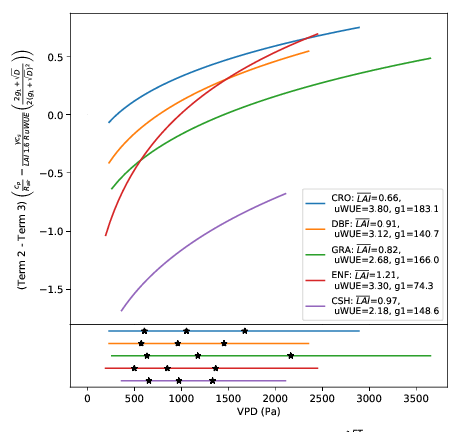
\includegraphics[width=3.5in]{sign.pdf}
    % \caption{}
  \end{figure}
\end{frame}

\begin{frame}{Summary of theory}
  \begin{itemize}
  \item We use \cite{Zhou_2016}'s uWUE to derive a new analytically tractable form of PM.
  \item This new analysis suggests that the ``tipping'' point for which atmospheric demand overwhelms plant response will be almost exclusively a function of VPD.
    \begin{itemize}
    \item For each PFT there will be a VPD$_{crit}$ above which atmospheric demand will dominate and ET will increase with VPD.
    \end{itemize}
  \item Plant types evolved to conserve water (CSH) have a higher VPD$_{crit}$ than plants evolved (or bred) to use water and prioritize GPP (CRO). Trees and grasslands are somewhere between these two extremes.
  \item Aerodynamic conductance scales the response, so plants with large surface roughness will be more likely to have a larger response as there is less resistance between the surface and the atmosphere.
  \end{itemize}
\end{frame}

\section{Results -n reality}
{ % all template changes are local to this group.
    \setbeamertemplate{navigation symbols}{}
    \begin{frame}[plain]{Idealized results - CRO}
        \begin{tikzpicture}[remember picture,overlay]
            \node[at=(current page.center)] {
                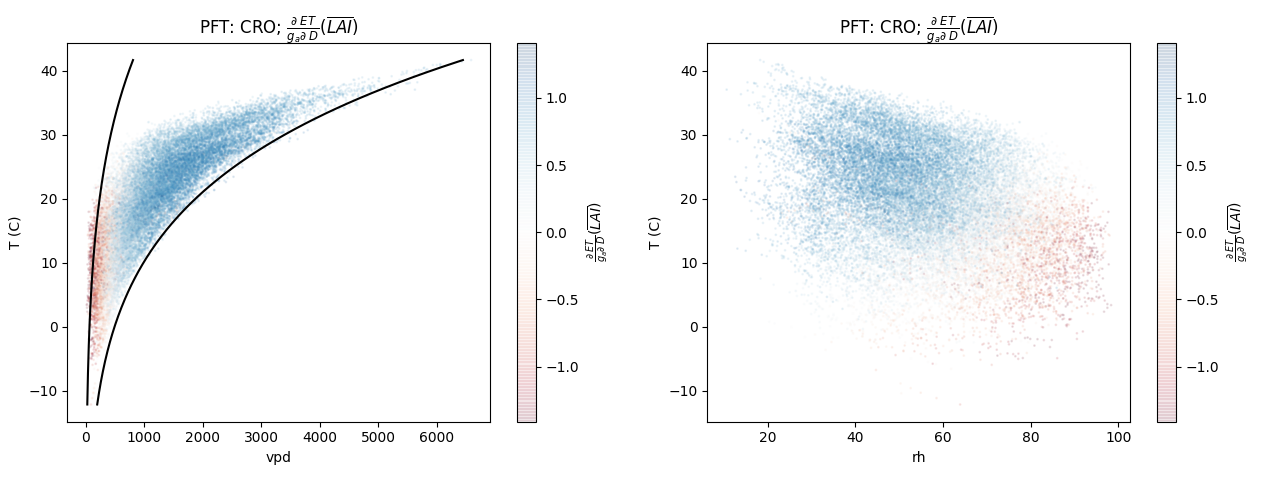
\includegraphics[width=\paperwidth]{cro_ideal.png}
            };
        \end{tikzpicture}
     \end{frame}
}

{ % all template changes are local to this group.
    \setbeamertemplate{navigation symbols}{}
    \begin{frame}[plain]{Results with uncertainty - CRO}
        \begin{tikzpicture}[remember picture,overlay]
            \node[at=(current page.center)] {
                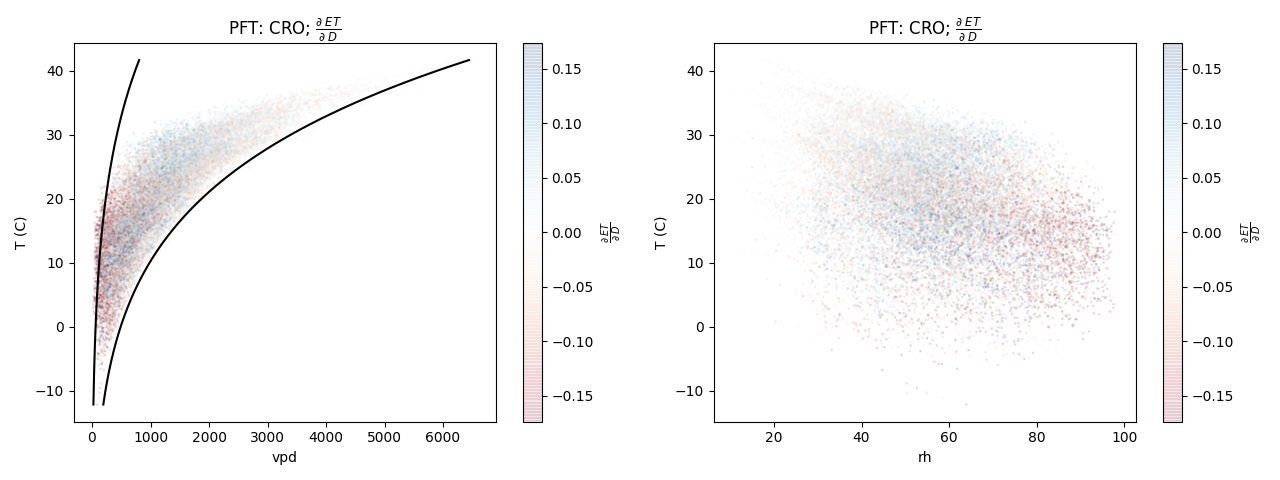
\includegraphics[width=\paperwidth]{cro.png}
            };
        \end{tikzpicture}
     \end{frame}
}

{ % all template changes are local to this group.
    \setbeamertemplate{navigation symbols}{}
    \begin{frame}[plain]{Idealized results - CSH}
        \begin{tikzpicture}[remember picture,overlay]
            \node[at=(current page.center)] {
                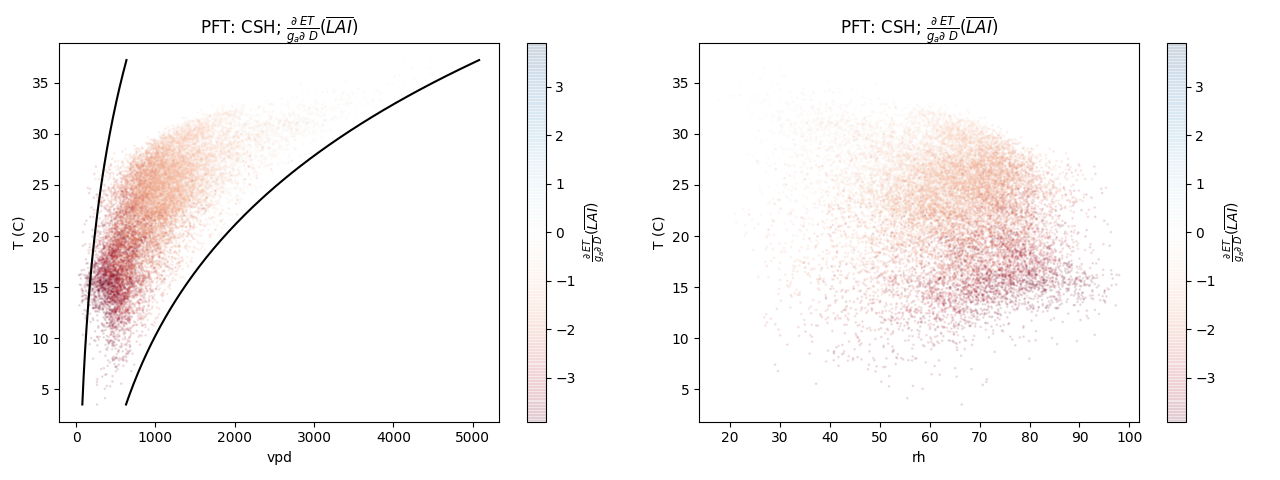
\includegraphics[width=\paperwidth]{csh_ideal.png}
            };
        \end{tikzpicture}
     \end{frame}
}

{ % all template changes are local to this group.
    \setbeamertemplate{navigation symbols}{}
    \begin{frame}[plain]{Results with uncertainty - CSH}
        \begin{tikzpicture}[remember picture,overlay]
            \node[at=(current page.center)] {
                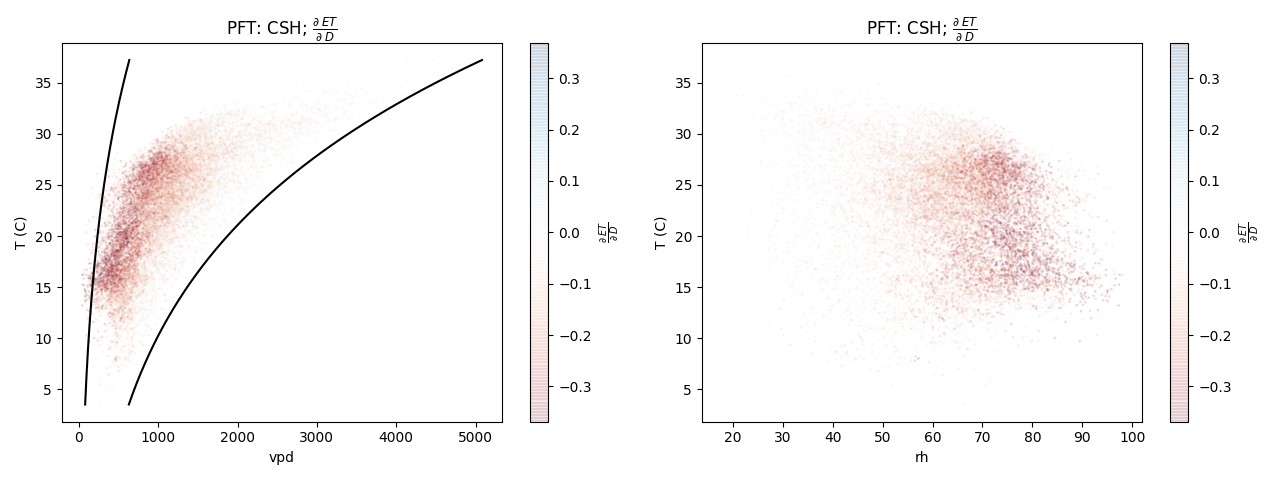
\includegraphics[width=\paperwidth]{csh.png}
            };
        \end{tikzpicture}
     \end{frame}
}

{ % all template changes are local to this group.
    \setbeamertemplate{navigation symbols}{}
    \begin{frame}[plain]{Idealized results - DBF}
        \begin{tikzpicture}[remember picture,overlay]
            \node[at=(current page.center)] {
                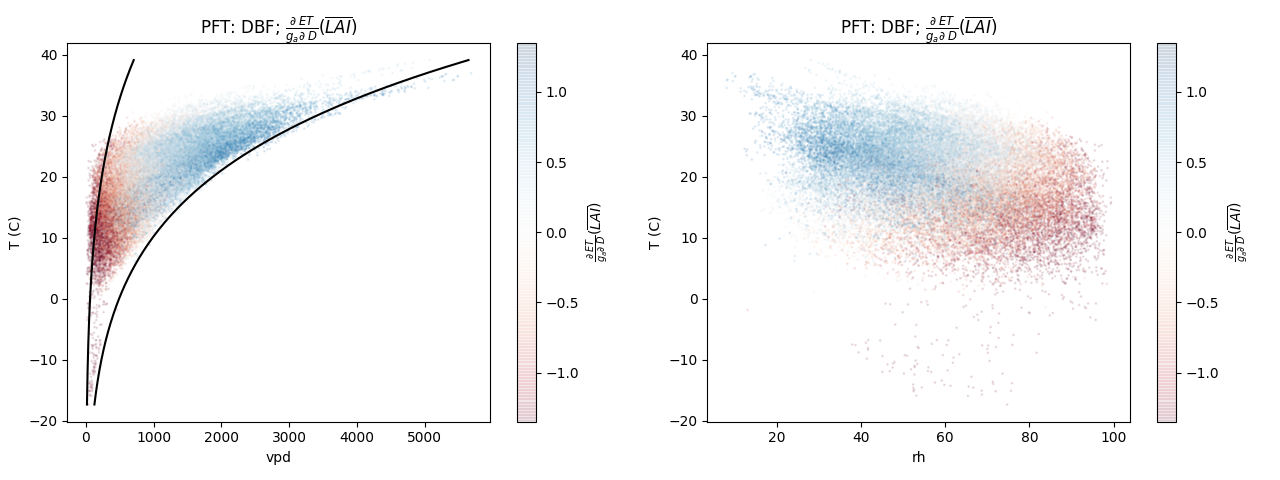
\includegraphics[width=\paperwidth]{dbf_ideal.png}
            };
        \end{tikzpicture}
     \end{frame}
}

{ % all template changes are local to this group.
    \setbeamertemplate{navigation symbols}{}
    \begin{frame}[plain]{Results with uncertainty - DBF}
        \begin{tikzpicture}[remember picture,overlay]
            \node[at=(current page.center)] {
                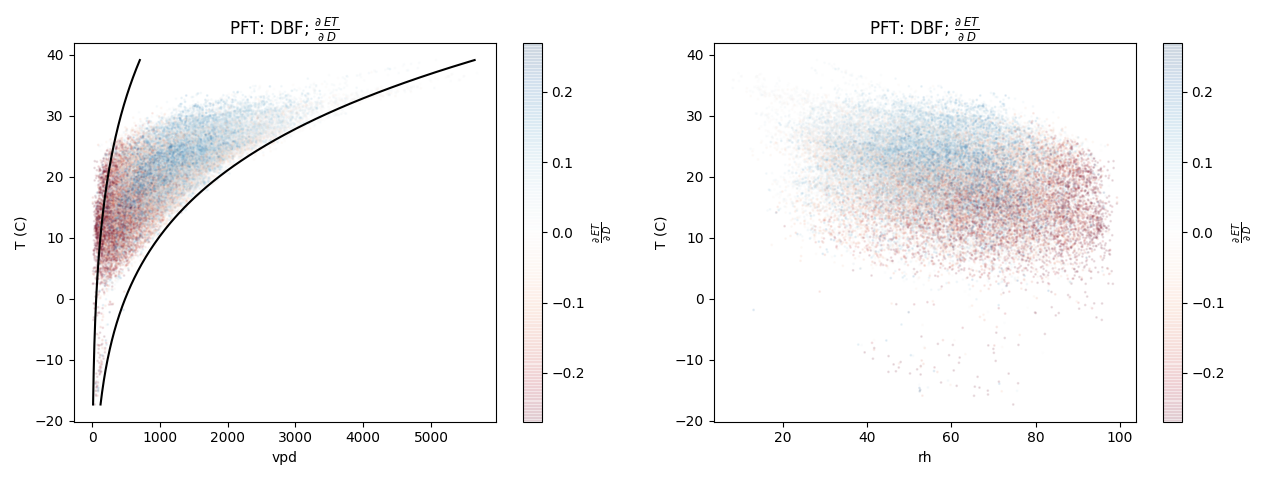
\includegraphics[width=\paperwidth]{dbf.png}
            };
        \end{tikzpicture}
     \end{frame}
   }

{ % all template changes are local to this group.
    \setbeamertemplate{navigation symbols}{}
    \begin{frame}[plain]{Idealized results - ENF}
        \begin{tikzpicture}[remember picture,overlay]
            \node[at=(current page.center)] {
                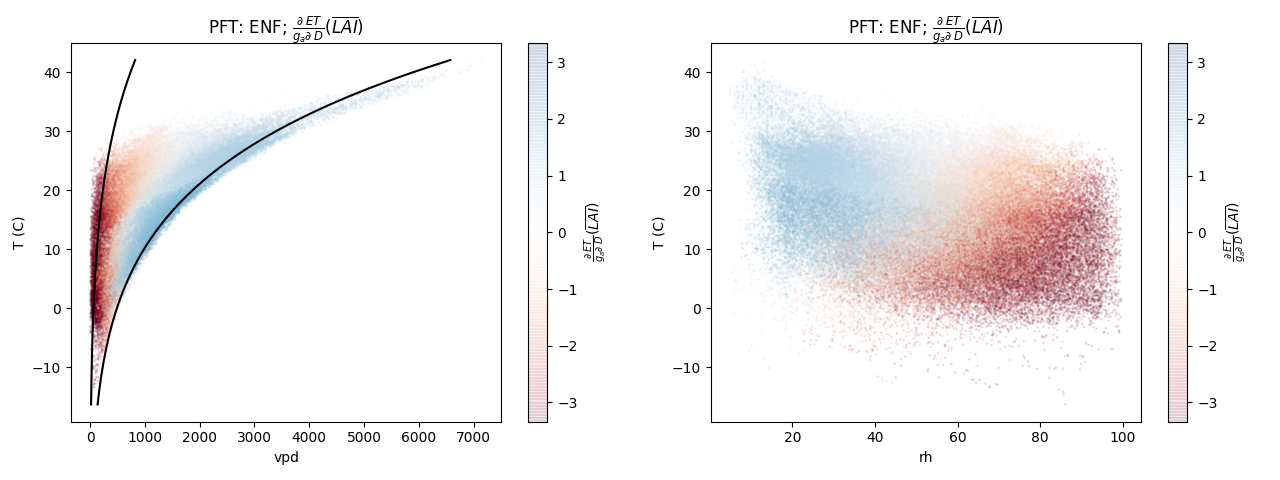
\includegraphics[width=\paperwidth]{enf_ideal.png}
            };
        \end{tikzpicture}
     \end{frame}
}

{ % all template changes are local to this group.
    \setbeamertemplate{navigation symbols}{}
    \begin{frame}[plain]{Results with uncertainty - ENF}
        \begin{tikzpicture}[remember picture,overlay]
            \node[at=(current page.center)] {
                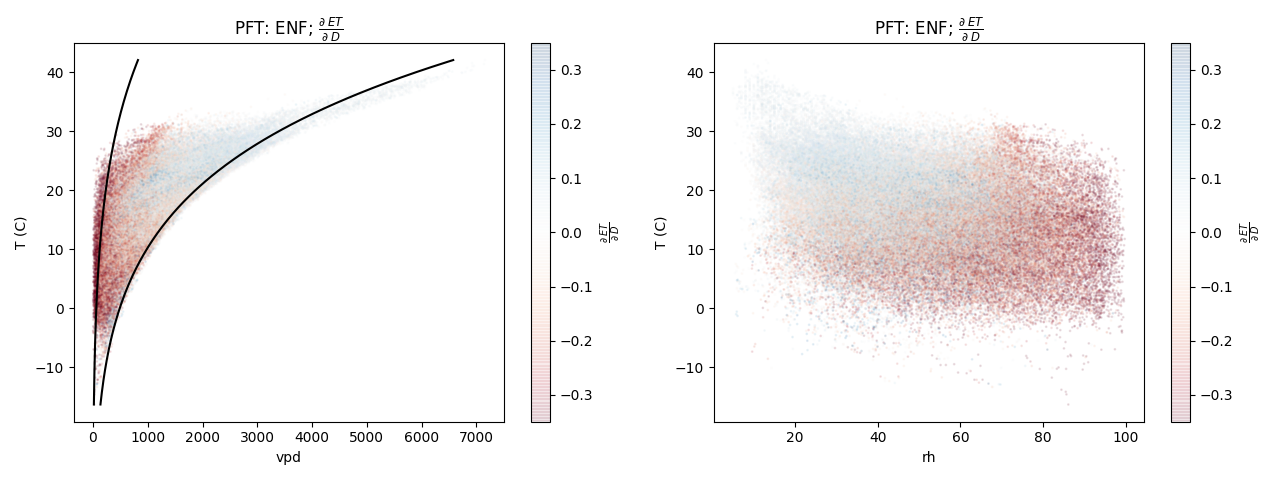
\includegraphics[width=\paperwidth]{enf.png}
            };
        \end{tikzpicture}
     \end{frame}
   }

{ % all template changes are local to this group.
    \setbeamertemplate{navigation symbols}{}
    \begin{frame}[plain]{Idealized results - GRA}
        \begin{tikzpicture}[remember picture,overlay]
            \node[at=(current page.center)] {
                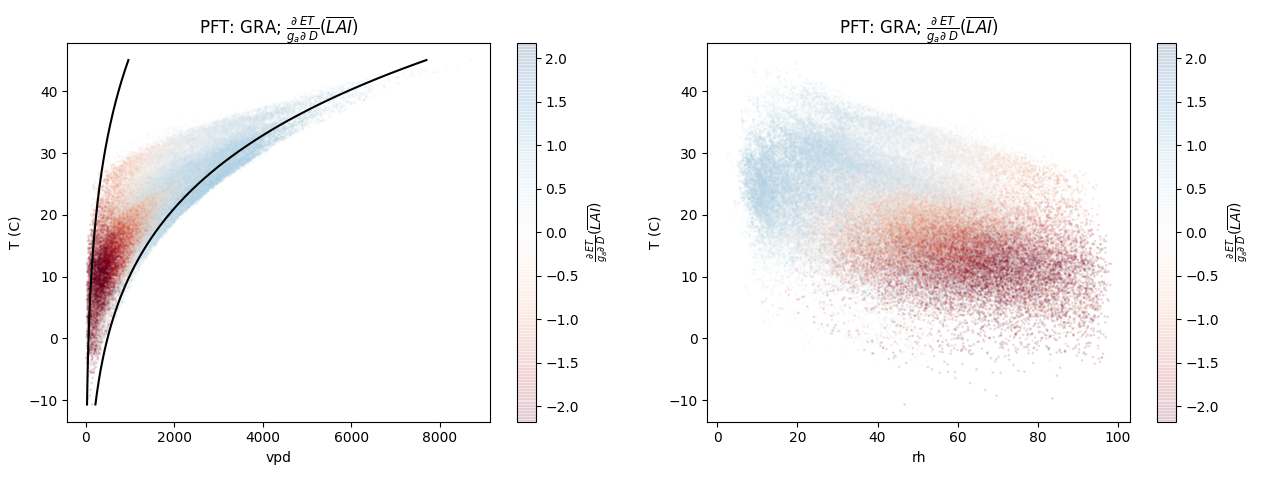
\includegraphics[width=\paperwidth]{gra_ideal.png}
            };
        \end{tikzpicture}
     \end{frame}
}

{ % all template changes are local to this group.
    \setbeamertemplate{navigation symbols}{}
    \begin{frame}[plain]{Results with uncertainty - GRA}
        \begin{tikzpicture}[remember picture,overlay]
            \node[at=(current page.center)] {
                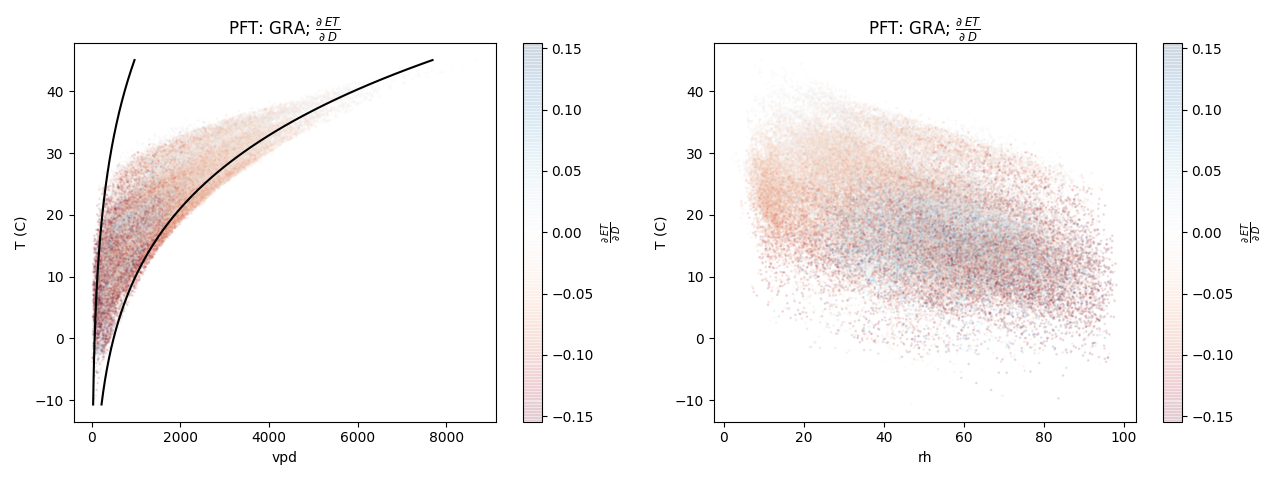
\includegraphics[width=\paperwidth]{gra.png}
            };
        \end{tikzpicture}
     \end{frame}
   }

   \begin{frame}{Summary statistics}
     \begin{table}
       \caption{Statistics of $\frac{\partial \; ET}{\partial \; D}$ as a function of PFT.}
       \centering
       \begin{tabular}{l c c}
         \hline
         PFT & $\overline{\frac{\partial \; ET}{\partial \; VPD}}$ & fraction $\frac{\partial \; ET}{\partial \; VPD} < 0.$ \\
         \hline
         CRO & 0.000853  & 0.473311\\
         CSH & -0.108234 & 0.931660\\
         DBF & -0.012727 & 0.461674\\
         ENF & -0.034087 & 0.534425\\
         GRA & -0.019637 & 0.631735\\
         \hline
         \multicolumn{2}{l}{}  
       \end{tabular}
     \end{table}
   \end{frame}
     
\section{Conclusions}
\begin{frame}{Summary}
  \begin{itemize}
  \item Theory finds that the ``tipping'' point for which atmospheric demand overwhelms plant response will be almost exclusively a function of VPD.  Plant types evolved to conserve water (CSH) have a higher VPD$_{crit}$ (and more negative ET response) than plants evolved (or bred) to use water and prioritize GPP (CRO).
  \item On average, ecosystem response to VPD follows roughly what we might expect: CRO (prioritize GPP) has positive ET response to VPD, while all others have a negative response. Ordering by increasing magnitude of negative response gives: DBF, GRA, ENF, CSH; which roughly correspond to expectations for increasing water conservation as a function of PFT.
  \item Uncertainty is high, especially for CRO and GRA. However, inclusion of uncertainty does not change the story for ENF or CSH.
  \end{itemize}
\end{frame}
  


\section{References}
\begin{frame}{References}
  \AtNextBibliography{\small}
  \printbibliography
\end{frame}


% \begin{table}
% \centering
% \begin{tabular}{l|r}
% Item & Quantity \\\hline
% Widgets & 42 \\
% Gadgets & 13
% \end{tabular}
% \caption{\label{tab:widgets}An example table.}
% \end{table}

\end{document}
